Convergence study mesh}
To create a mesh that is fine enough to give representative results and also coarse enough to limit the processing time, a convergence study is conducted. 
Since the cavity has the most complex structure and might possibly result in a complicated stress, a meshing strategy should be used to reduce the error in that region. Therefore, local adaptive mesh refinement was applied to the RVE. To find the minimum size of the mesh different meshes where analyzed with a approximate global size of 0.05 and a constant curvature control of 0.01. The convergence study showed an optimal minimum size control of approximately 0.003. Figure \ref{fig:Convergencestudysmallest} shows the number of elements related to the results in E1 E2 and E3. E3 seems to be most sensitive to changes, which is logical according to the shape of the cavity, which deviate most of the stresses.

\begin{figure}[H]
    \centering
    \includegraphics[width=0.40\textwidth]{chapter_6_Elasticmodelling/figures/Convergeancestudyforsmallest.png}
    \caption{Convergence study for minimum size control}
    \label{fig:Convergencestudysmallest}
\end{figure}

A second convergence study was done to determine the maximum global size. The maximum global size was altered from a coarse mesh (0.05) towards finer meshes. The convergence study in figure \ref{fig:Convergencestudyglobal} indicates that a global size of approximately 0.02 gives representative results.

\begin{figure}[H]
    \centering
    \includegraphics[width=0.40\textwidth]{chapter_6_Elasticmodelling/figures/Convergeancestudyforglobalmesh.png}
    \caption{Convergence study for approximate global size}
    \label{fig:Convergencestudyglobal}
\end{figure}

Finally, multiple stacked RVE's where studied to determine the minimal amount of RVE's needed to acquire consistent results. When stacking 2 by 2 (figure \ref{fig:RVE22}) and 3 by 3 RVE's no variation in results where found, therefore we can assume that a single RVE will give representative results).

\begin{figure}[H]
    \centering
    \includegraphics[width=0.40\textwidth]{chapter_5_RVEmodel&amp;verification/figures/ScreenshotRVE22.png}
    \caption{2 by 2 stacked meshed RVE's}
    \label{fig:RVE22}
\end{figure}

The resulting RVE with a global element size of 0.02mm and a minimal element size of 0.003 gives consistent results and can be observed in figure \ref{fig:RVEfinal}. The total processing time for this mesh is 1.7 minutes and has 14060 elements, this is similar to the mesh found in literature (. The results will be presented in the section "Results". 

\begin{figure}[H]
    \centering
    \includegraphics[width=0.40\textwidth]{chapter_5_RVEmodel&amp;verification/figures/RVEcmon.png}
    \caption{Resulting meshed RVE with 0.02mm global elements and 0.003mm minimal elements}
    \label{fig:RVEfinal}
\end{figure}

\subsection{Tensile tests}
To verify the model, where the goal is to achieve a better response with this model compared to the models from the literature, multiple tensile tests are conducted. These tensile tests are conducted according to the standardization described in chapter \ref{chp:lit_rev}. The ISO 527 norm is applied for the tensile testing, which includes a “dogbone profile” for polymer parts and has a test set of 5 specimens per case. The test was displacement driven with an elongation of 2mm/min. An extensometer was used to have a more precise measurement of the elongation. The machine used was [Machine used] and the results are processed with the [software] at the materials lab of the TU Delft. 
Since there are no strict standards for the process of FFF test samples, the standards described in chapter \ref{chp:lit_rev} are applied for this case. In table [table] the process parameters are shown for the FFF parts in different direction.  These parts are all produced on an Ultimaker S5 with Ultimaker provided ABS. Parts with the same process parameters have been analyzed with optical microscopy in chapter \ref{chp:4meso}. 
In this experiment 5 samples in the 3 principle directions were tested, produced in the yx[0], xy[0] and zy[0] direction. The samples where printed in the same print process, filling the majority of the print bed. Alongside this print job a test specimen in the yx[0] was produced to observe the related mesostructured. With these tests the anisotropy of FFF parts can be determined.

The point of failure of the dogbones was not at the desired point. The dogbones are designed to break at the thinner part of the specimen, if the material is uniform along the dogbone, the distribution along the thin part should be equal. The tested parts however, failed all, with the exception of 3 of the 15 specimen, at the (beginning) of the fillet. Also, most of the parts experienced a brittle failure. In figure 2 specimen are shown for every loading direction.

\begin{figure}[H]
    \centering
    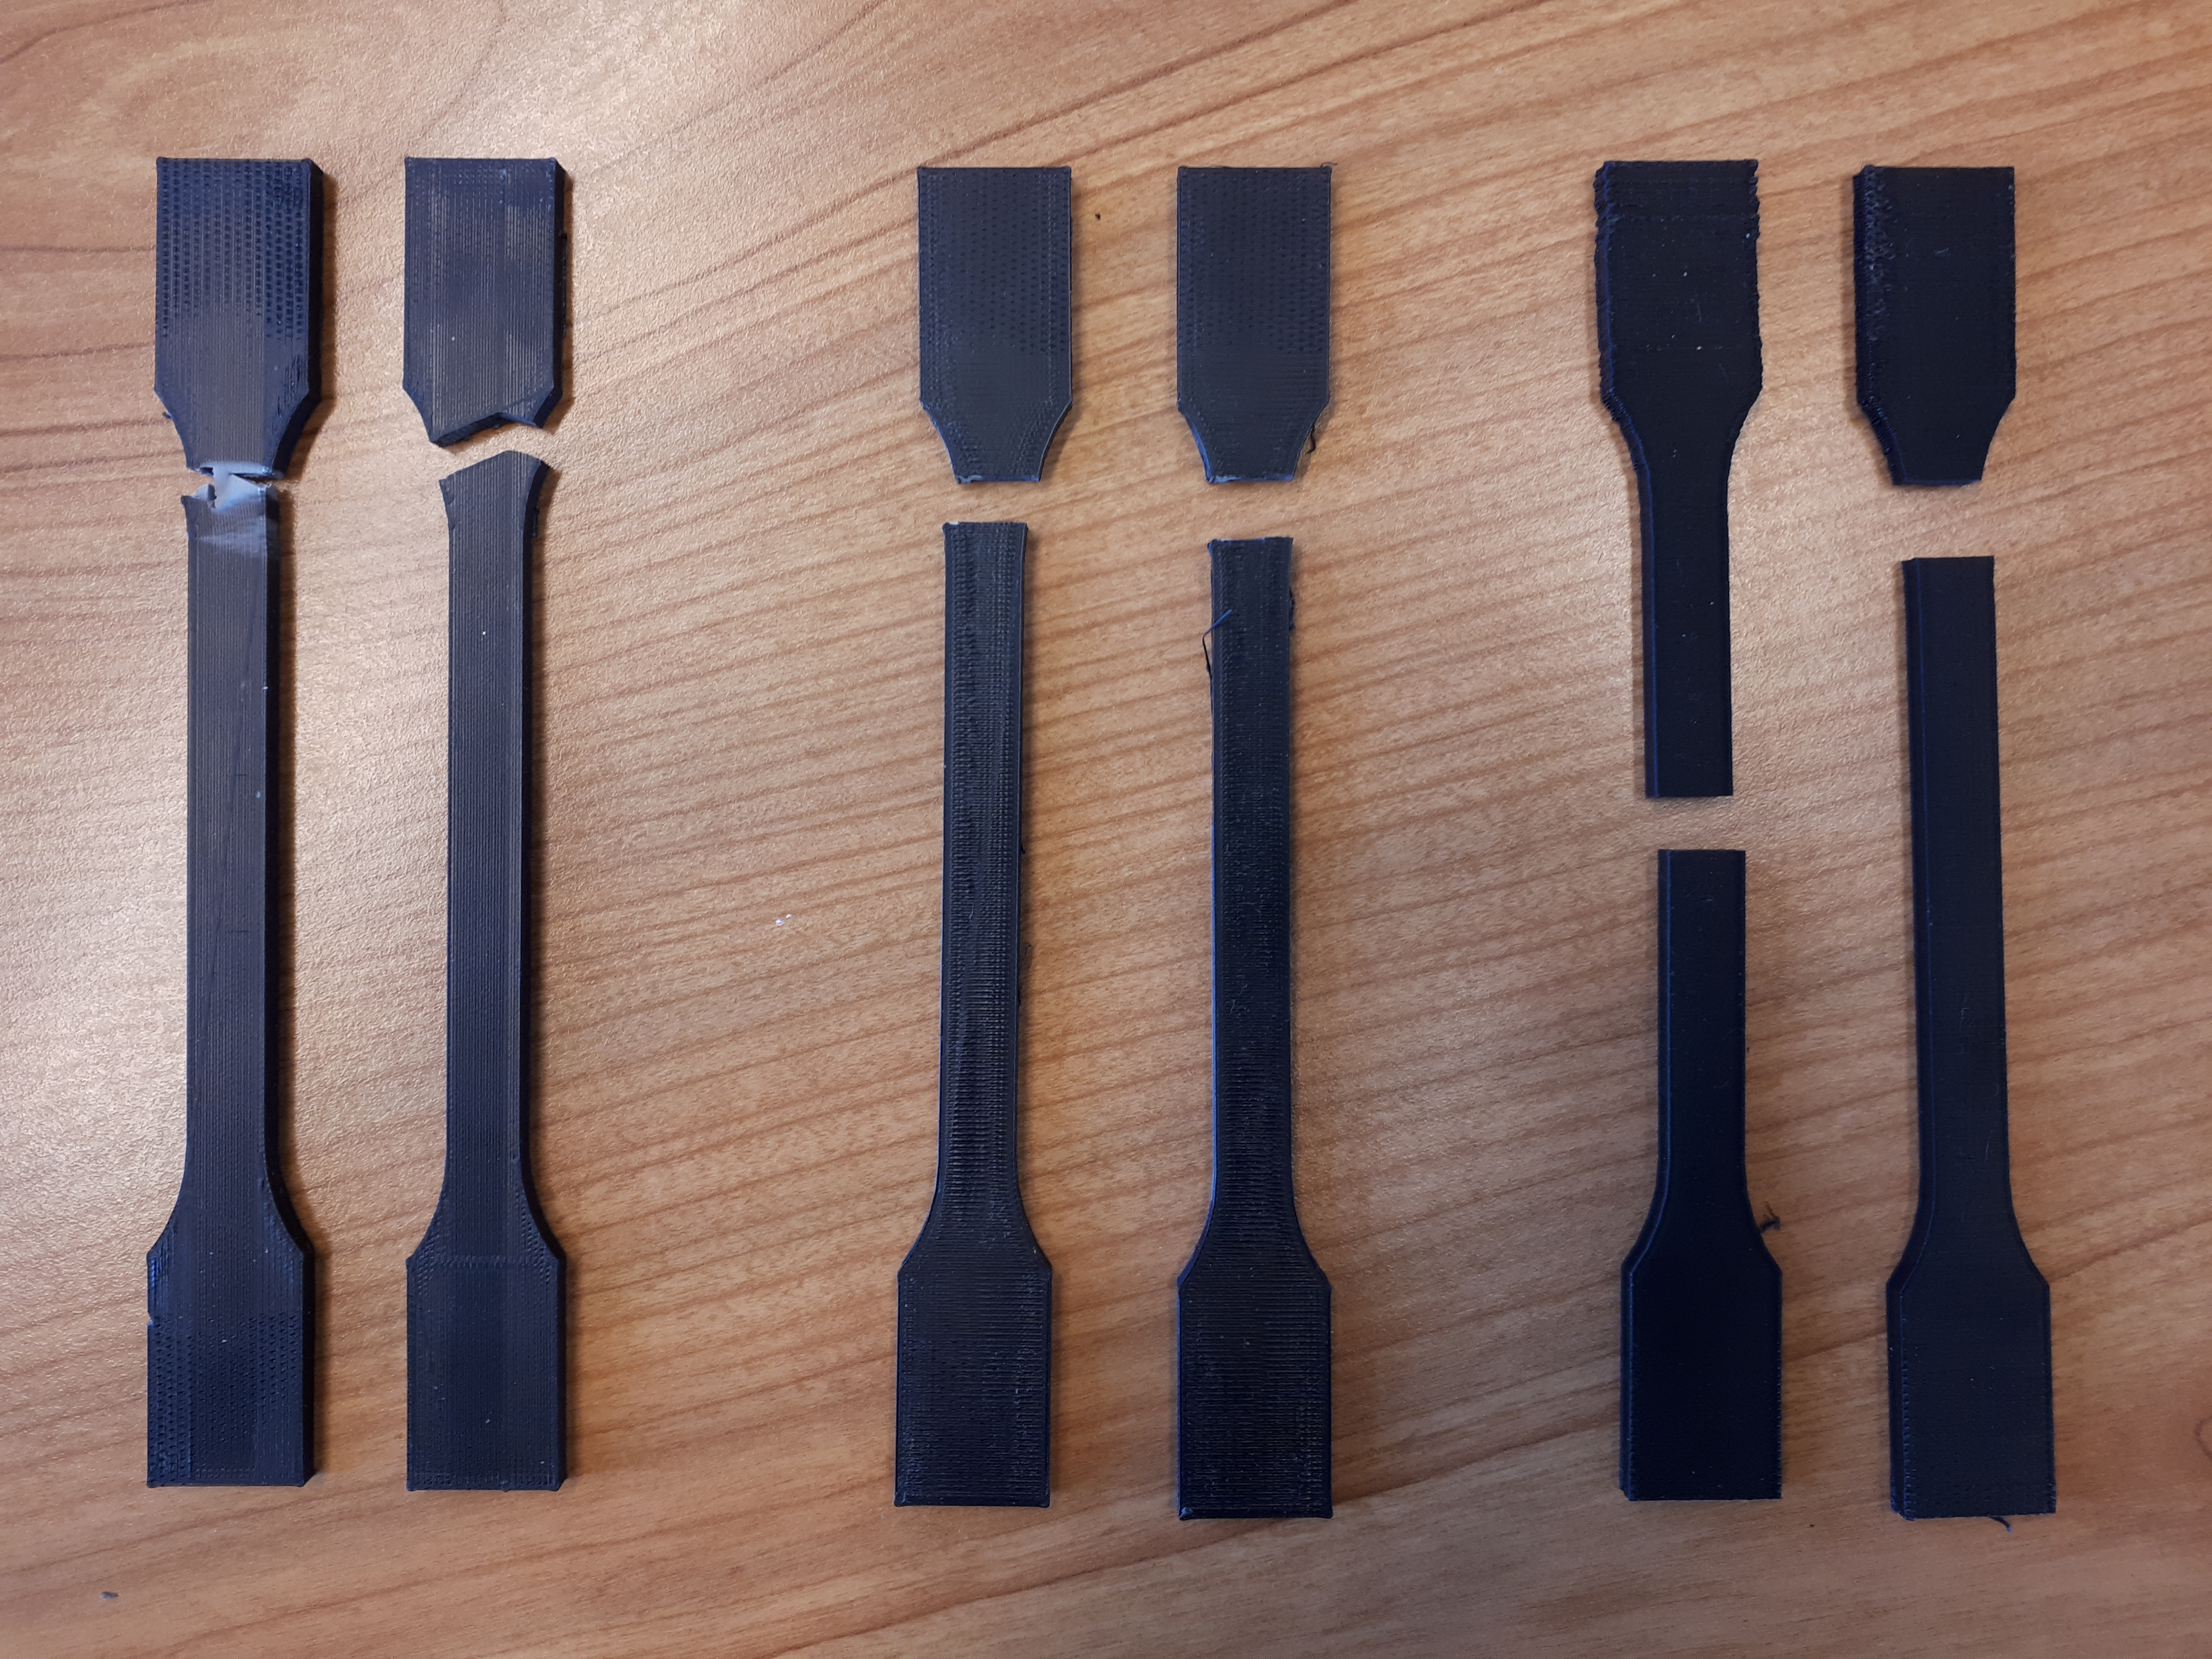
\includegraphics[width=0.80\textwidth]{chapter_5_RVEmodel&amp;verification/figures/specimen.jpg}
    \caption{Tested specimen, left yx[0], middle xy[0], right zy[0]}
    \label{fig:specimen}
\end{figure}
%%%% ADDING 
 \pagebreak[4]


\section{Results}
\subsection{RVE model}
The results of the RVE homogenization model are presented in figure \ref{fig:RVEresults}. The three directions are the 1 2 and 3 principle directions, which are respectively yx[0] xy[0] and zy[0].

\begin{figure}[H]
    \centering
    \includegraphics[width=0.80\textwidth]{chapter_5_RVEmodel&amp;verification/figures/E-moduliRVEUltimakerABS02_04[0]n.png}
    \caption{E-moduli for a 0.2mm x 0.4mm x 0.4mm RVE}
    \label{fig:RVEresults}
\end{figure}

The homogenization is calculated by applying a deformation of 0.03 in 6 different directions and averaging the stresses. The different deformations can be seen in figure \ref{fig:deformations}.

\\
\begin{figure}
\centering
  \begin{subfigure}[b]{0.40\textwidth}
    \includegraphics[width=\textwidth]{chapter_5_RVEmodel&amp;verification/figures/p1.png}
    \caption{Tensile strain 11 direction}
    \label{fig:1}
  \end{subfigure}
  %
  \begin{subfigure}[b]{0.40\textwidth}
    \includegraphics[width=\textwidth]{chapter_5_RVEmodel&amp;verification/figures/p2.png}
    \caption{Tensile strain 22 direction}
    \label{fig:2}
  \end{subfigure}
  \\
    \begin{subfigure}[b]{0.40\textwidth}
    \includegraphics[width=\textwidth]{chapter_5_RVEmodel&amp;verification/figures/p3.png}
    \caption{Tensile strain 33 direction}
    \label{fig:3}
  \end{subfigure}
  %
  \begin{subfigure}[b]{0.40\textwidth}
    \includegraphics[width=\textwidth]{chapter_5_RVEmodel&amp;verification/figures/p4.png}
    \caption{Shear strain 12 direction}
    \label{fig:4}
  \end{subfigure}
  
  \begin{subfigure}[b]{0.40\textwidth}
    \includegraphics[width=\textwidth]{chapter_5_RVEmodel&amp;verification/figures/p5.png}
    \caption{Shear strain 13 direction}
    \label{fig:1}
  \end{subfigure}
  %
  \begin{subfigure}[b]{0.40\textwidth}
    \includegraphics[width=\textwidth]{chapter_5_RVEmodel&amp;verification/figures/p6.png}
    \caption{Shear strain 23 direction}
    \label{fig:2}
  \end{subfigure}
  \\

  
  \caption{Different deformation cases for the calculation of the homogenized properties}
    \label{fig:deformations}
\end{figure}

 \pagebreak[4]




\subsection{Tensile test}
The results of the tensile test are presented in figure \ref{fig:RVEresults}. The three directions are the 1 2 and 3 principle directions, which are respectively yx[0] xy[0] and zy[0].

\begin{figure}[H]
    \centering
    \includegraphics[width=0.80\textwidth]{chapter_5_RVEmodel&amp;verification/figures/Tensileresults.PNG}
    \caption{Results in 3 principle directions}
    \label{fig:tensileresults}
\end{figure}

In table \ref{tab:tensileresults} the material properties in the different directions are presented.
\begin{center}
 \begin{tabular}{||c c c c||} 
  \caption{Mechanical properties obtained from tensile tests \label{tab:tensileresults}}\\
  
 \hline
 Direction & E [MPa] (mean) & \sigma_y [MPa] (mean) & \epsilon_y [\%] (mean) \\ [0.5ex]
 \hline\hline
 Injection moulded \cite{TechnicalUM} & 2030 & 43.6 & 4.8 \\ 
 \hline
 1 & 2019 & 31.5 & 1.8 \\
 \hline
 2 & 1974 & 30.8 & 1.9 \\
 \hline
 3 & 1793 & 16.3 & 1 \\
 [1ex] \hline
\end{tabular}
\end{center}

\section{Discussion}
The results of the RVE homogenization model and tensile tests both give similar results compared with the findings in the literature. Before we can compare both of the results some points need to be adressed.

The design for the RVE is based on the micrographs and slicing knowledge discussed in chapter \ref{chp:4meso}. The material used in the RVE is homogeneous and isotropic, and will generate an insotropic response due to the presence of the cavity. In reality there will probably be different regions with different mechanical properties due to the bonding between roads. The mechanical response that is generated is therefore probably an overestimation of the reality. To create a better representation, cohesive elements or regions should probably be applied.

The material currently used for the RVE homogenization is based on the Ultimaker ABS TDS \cite{TechnicalUM} which gives a "Typical" injection moulded value of 2030 MPa and a printed value of 1618.5 MPa with 90\% infill. Other filament brands (Stratasys) used in the literature indicate a significant difference which has been tested by tensile testing a monofilament. The tested value (2230 MPa) was in reasonable agreement with the provided value by Stratasys (2400 MPa) \cite{Rodriguez2001MechanicalInvestigation}. Since injection moulded properties can significantly vary with the filament, the value provided by Ultimaker can be misleading. Nonetheless, this value was still used as input material for the RVE homogenization, something to consider. 

During the tensile test the dogbones failed at an undesired spot, at the fillets of the specimen. This can have several causes or a combination of them. FFF produced parts have inherent surface surface roughness, artifacts or other anomalies. This can be due to the road deposition process, which creates a rough surface or a defect in the process where too much or too little material is deposited at a wrong spot. These defects can induce stress concentrations, since the change of geometry are points that are more prone to this effect, stress concentrations are likely to occur here. This can be partially solved in some cases by adding wall layers, which will produce a more smooth road. Another possibility is the theory that stress is not homogeneously divided between roads, if a narrowing of roads occur stress concentrations at the edges might induce more stress concentration. Therefore, the full capacity of the material is not achieved, and a pre-mature brittle fracture will result. A different test method (ASTM D3039) used by Rodriguez \cite{Rodriguez2001MechanicalInvestigation}, which is more appropriate for long fiber composites, gives a much more ductile response in the xy[0] direction than the specimen tested in this experiment. 

If we compare the results from the RVE homogenization with the results obtained with the tensiles test, it seems that the tensile test performs significantly better in the 3 direction (20\%), and slightly better in the 1 and 2 directions (2\%). Since we considered that due to the lack of cohesive elements the RVE model over-performs and due to the stress concentration the tensile tests might under-perform, there must be another cause for this discrepancy. There might be two different causes, the first might be a applied E-modulus for the RVE model that is too low compared with the reality, the other possibility might be a too large or wrong cavity design, which results in lower properties.

\subsection{Conclusion and recommendations}
If the results for elliptical RVE's are compared with the RVE proposed in this work, it is clearly noticeable that the simulation results for the adjusted RVE are much closer to the tested specimen than the elliptical RVE. This is especially apparent for the 2 direction, which has a higher E-modulus due to the absence of the lower cavity. 

The results from the RVE model and tensile test are in the same range, but differ nonetheless significantly in the 3 direction. In the discussion different possible causes are discussed. The probability that the cause is in the RVE model is highest and must therefore be adjusted to have a better response, this can be either iterations to match the cavity better or a test to test the ABS mono-filament to determine the bulk modulus. Hypothetically, there is a slight difference between the porosity shown in figure \ref{fig:Mesoresults} and the RVE design in figure \ref{fig:RVEsimple}, the horizontal corners are quite long compared to the micrographs, which might result in a worse response in the 3 direction.  

Besides, there is large room for optimization in the tensile testing procedure. The current response is very brittle and does not fully load the specimen in the thin region. To improve this, another test method could be used which does not implement change in thickness of the part. Also, it has been noted in the work of Rodriguez that increasing the loading speed might give a better ductile response \cite{Rodriguez2001MechanicalInvestigation}.

When these issues have been addressed, additional tests can be done to inspect the cohesive properties of the layers. Since there is no clear understanding of the literature on behalf of the behaviour of sintering, a specimen with different road colors could be printed and inspected with optical microscopy. Based on this information the geometry of implemented cohesive elements or regions can be defined, subsequently the properties of these elements should be determined based on experimental data and theoretical substantiation. 

A following step could either be analyzing the plastic deformation of the RVE, or determining the yield strength conducting more complex experiments to determine the yield surface coefficients. For the former option a well defined RVE model should be formulated.





\graphicspath{{chapter_4/figures/}}
\graphicspath{{chapter_2/figures/}}% path to the figures folder of this chapter